\documentclass[a4paper,11pt,twoside]{report}
\usepackage[utf8]{inputenc}

% geometry for the documents in this dir.
\usepackage[a4paper,includemp,
      scale={0.9,0.9},
      includeheadfoot,
      bindingoffset=1.5cm]{geometry}
% This is an annotated latex definition file.
% You can give it any name as long as its inputted somewhere
% in your code.
% You may even put it in a directory other then the current
% as long as that directory is in the TEXINPUTS path.
% Comments start with a % as you a seeing right now. Otherwise look
% to the left.
% font of the times family
%\usepackage{palatino}
\usepackage{lmodern}
% make linenumbering possible for reviewing
\usepackage[pagewise,mathlines,displaymath]{lineno}
% use the pdftex graphics extensions
\usepackage{graphicx}
\usepackage{wrapfig}
% to make the headers and footers look nice
\usepackage{xcolor,fancyhdr}
% allow drawing with tikz
\usepackage{tikz}
% allow compact lists etc.
\usepackage{enumitem}
% make the header (and footer) span the whole printable area
\addtolength\headwidth\marginparwidth
\addtolength\headwidth\marginparsep
\pagestyle{fancy}
\usepackage[all]{svn-multi}
\svnRegisterAuthor{879417}{Pieter van den Hombergh}

% \usepackage{svn}
\newcommand\TheFile{mydefs.tex}
\newcommand\Code[1]{\textbf{\texttt{#1}\ }}
%%
% to get version information in files, include the following lines in
% each document 
% and renewcommand\TheFile to something like \renewcommand\TheFile{main.text}
%\renewcommand\footrulewidth{1pt}
% put revision control info in the footer
% the vspace compensates for the space taken up by the logo on the right hand.
% I like a fontys color in my header
\definecolor{purple}{rgb}{0.21,0,0.21} % a darkish purple
\renewcommand\headrule{%
  {\color{purple}%
    \hrule height 2pt width \headwidth
    \vspace{1pt}%
    \hrule height 1pt width \headwidth
    \vspace{-4pt}%
  }%
}%
\renewcommand\footrule{
  {\color{purple}%
    \hrule height 1pt width \headwidth
    \vspace{1pt}%
    \hrule height 2pt width \headwidth
    \vspace{2pt}%
  }%
}
% do not indent pars, increase parskip
\setlength\parindent{0pt}
\setlength\parskip{0.5em}
% my own itemize: a bit less spacy then the default
\newenvironment{Itemize} {
  \begin{itemize}{}%
    \setlength\topsep{0ex}%
    \setlength\parskip{0ex}%
    \setlength\partopsep{0em}%
    \setlength\parsep{0em}%
    \setlength\itemsep{0em}%
    }%
  {\end{itemize}}
% make the head a bit heigher
\setlength\headheight{16pt}
\setlength\footskip{60pt}
%%
% This macro '\define' puts the argument in em 
% and in boldface in the margin.
\newcommand{\define}[1]{% 1 argument
  \mbox{}{\textit{#1}}% italics or em
  \marginpar{\raggedright% no adjust
    \bfseries\hspace{0pt}#1}% bold
} % end of macro

%%
% At start of pages, define sometimes puts the material in the wrong margin
% in that case use this fix.
\newcommand{\fixdefine}[1]{\mbox{}{\textit{#1}}%
  \reversemarginpar\marginpar{\bfseries\hspace{0pt}#1}\normalmarginpar}
% to display source code like things
\usepackage{listings}
\lstset{numbers=right} % to get out of the way with document line numbers
% to be able to 'on this page' and the like
\usepackage{varioref}
% to put a nice quote with the chapter
\usepackage[avantgarde]{quotchap}
\renewcommand\chapterheadstartvskip{\vspace*{-5\baselineskip}}
%select Helvetica for title and quote
\usepackage{helvet}
\renewcommand\sectfont{\sffamily\bfseries}

%% example
%\begin{savequote}[10cm]
% \sffamily
%some text
%\end{savequote}
% needed for inclusion of gnumeric table
\def\inputGnumericTable{}
%% 
\usepackage{array}    
\usepackage{longtable}
\usepackage{calc}     
\usepackage{multirow} 
\usepackage{hhline}   
\usepackage{ifthen}   
%%
% Fancy headers are used
% To make the footer appear on chapter pages too,
% we redefine the fancypagestyle plain
\fancypagestyle{plain}{%
  \fancyhf{} % clear all  
  \fancyfoot[RO,LE]{\vspace{-1.2cm}%
  File: \svnkw{Filename}\\%
  Author: \svnFullAuthor*{\svnfileauthor}\\%
  Revision: \svnrev, \svnyear-\svnmonth-\svnday\ \svnhour:\svnminute\\
}
  \fancyfoot[RE,LO]{
\includegraphics[width=2cm]{figures/fon000_00c.pdf}}
  \fancyfoot[C]{\bfseries\thepage}
  \renewcommand\headrule{}%
}% end of redef fancypagestyl plain
% Define my own fancy headers and footers  
\fancyhead{}
\fancyhead[RO]{\rightmark} % display section name
\fancyhead[LE]{\rightmark}
\fancyfoot[RO,LE]{\vspace{-1.2cm}%
  File: \svnkw{Filename}\\%
  Author: \svnFullAuthor*{\svnfileauthor}\\%
  Revision: \svnrev, \svnyear-\svnmonth-\svnday\ \svnhour:\svnminute\\
}
% logo in footer
\fancyfoot[RE,LO]{
\includegraphics[width=2cm]{figures/fon000_00c.pdf}}
\pagestyle{fancy}
\usepackage{fontyscoverpage}
%%
% For a watermark on each page:
\usepackage{eso-pic} % needed package
% Draw a DRAFT through the text.
% for other text renewcommand the next command
\newcommand\watermarktext{Draft}
% You could make this depend on the status of the files.
\makeatletter
  \AddToShipoutPicture{%
    \setlength{\@tempdimb}{.5\paperwidth}%
    \setlength{\@tempdimc}{.5\paperheight}%
    \setlength{\unitlength}{1pt}%
    \put(\strip@pt\@tempdimb,\strip@pt\@tempdimc){%
      \makebox(0,0){\rotatebox{55}{% for longer texts you might want to increase this angle
          \textcolor[gray]{0.85}{% the higher the number, the lighter the text
            \fontsize{8cm}{8cm}% Fit this font to the text
            \sffamily
            \selectfont{\watermarktext}}}}
    }
}
\makeatother
\lstdefinelanguage{BibTeX}
  {keywords={%
      @article,@book,@collectedbook,@conference,@electronic,@ieeetranbstctl,%
      @inbook,@incollectedbook,@incollection,@injournal,@inproceedings,%
      @manual,@mastersthesis,@misc,@patent,@periodical,@phdthesis,@preamble,%
      @proceedings,@standard,@string,@techreport,@unpublished%
      },
   comment=[l][\itshape]{@comment},
   sensitive=false,
  }

% thenext comments are inserted by Emacs, that uses it 
% to process this latex file
%%% Local Variables: 
%%% mode: latex
%%% TeX-master: t
%%% End: 

%% If you need a bibliography
%
% \usepackage[square]{jurabib}
% \bibliographystyle{jurabib}
\usepackage[backend=biber,
style=alphabetic,natbib=true,
sorting=nyt]{biblatex}
\addbibresource{bibtex/latex.bib}
\addbibresource{bibtex/SEN2Bibliography.bib}
\svnidlong{$HeadURL: https://www.fontysvenlo.org/svnp/879417/latexcolloquium/trunk/latexsample/main.tex $}%
{$LastChangedDate: 2014-11-16 16:03:56 +0100 (zo, 16 nov 2014) $}%
{$LastChangedRevision: 62 $}%
{$LastChangedBy: 879417 $}
\svnid{$Id: main.tex 62 2014-11-16 15:03:56Z 879417 $}

\renewcommand\TheFile{main.tex}

%
% hyperef last, after all other packages
% this allows you to add hyperlinks in the document.
% It makes viewing it with e.g. Adobe acrobat very nice.

\usepackage[pdftex,colorlinks=false,
    pdfstartview=FitV,
    linkcolor=blue,
    citecolor=blue,
    urlcolor=blue,
    ]{hyperref}
\pdfinfo{
  /Title      (Sample latex document)
  /Author     (Pieter van den Hombergh 879417)
  /Keywords   (latex documentation graphics math listings)
}


% every document needs a start and an end
\author{Pieter~van~den~Hombergh\\879417}
\title{Sample \LaTeX\ document}
\begin{document}
% lets have a default title page
\pagenumbering{roman}
\AddToShipoutPicture*{\CoverBackgroundPic}

{
\setlength{\unitlength}{1mm}
\begin{picture}(0,0)(25,270)
\put(40,75){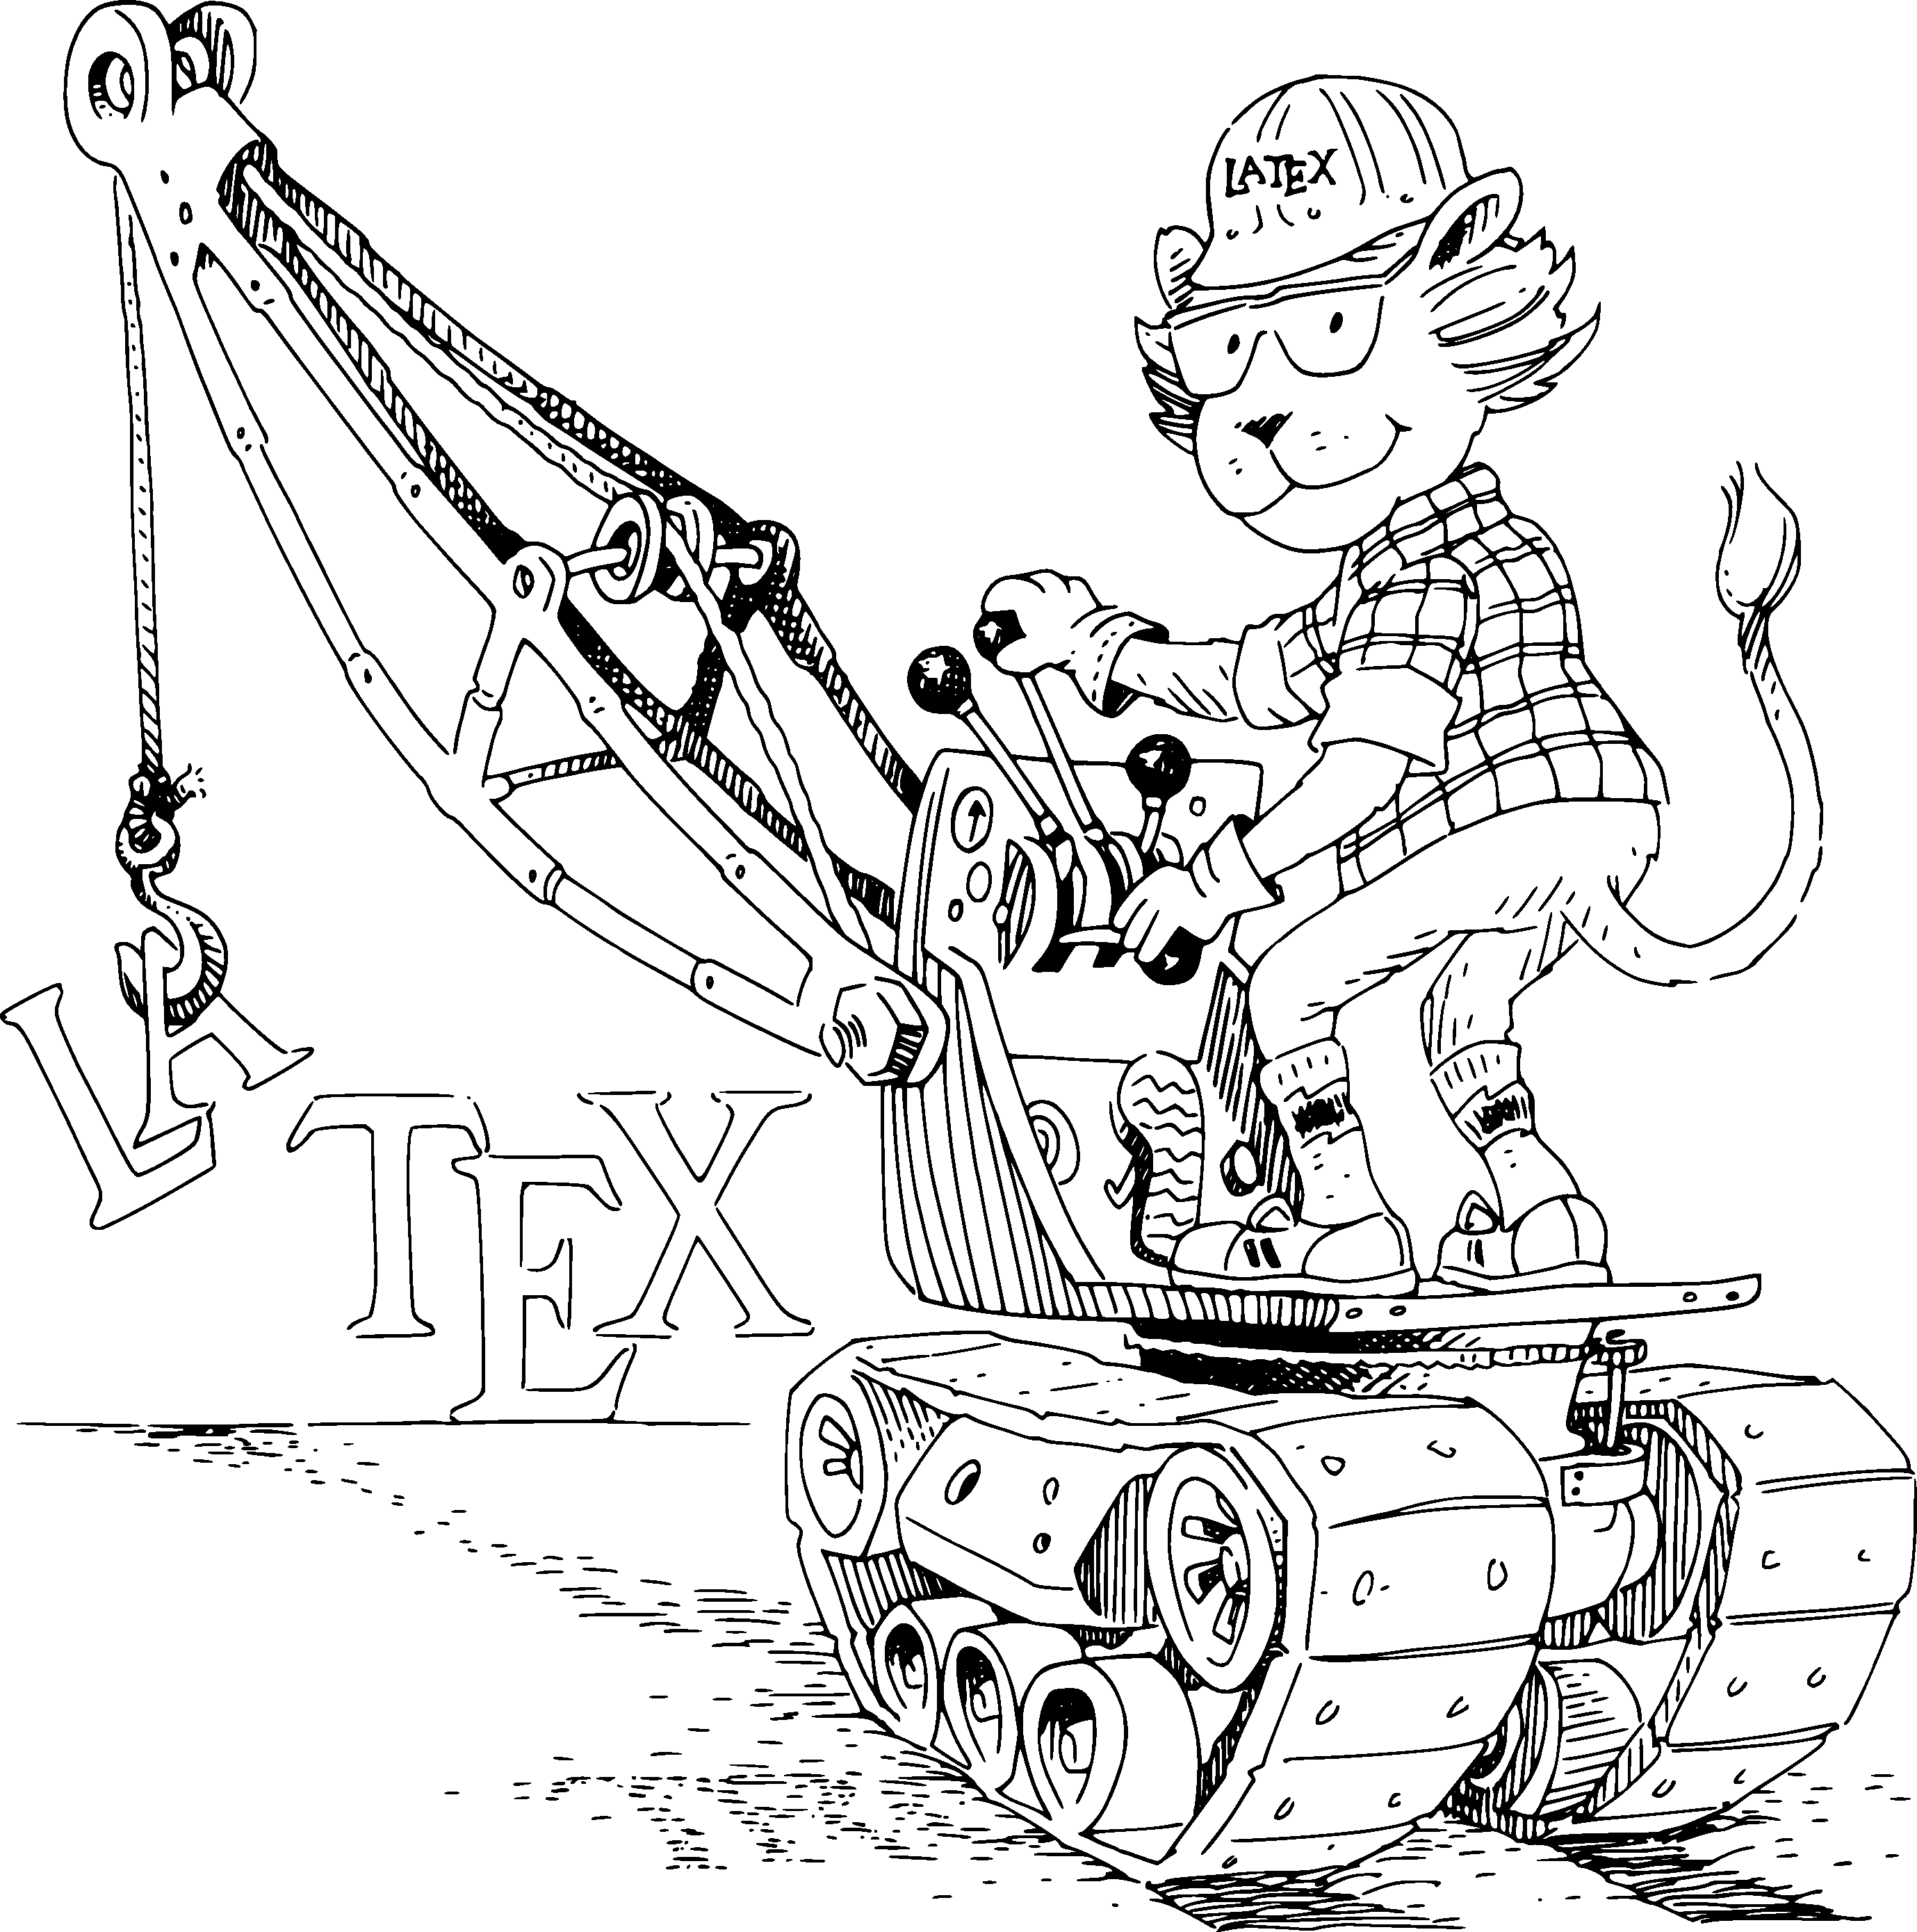
\includegraphics[width=140mm]{figures/latexlion.pdf}}
\put(140,69){\color{gray}drawing by Duane Bibby}

  \put(10,10){\begin{minipage}[b]{\textwidth}
    \parindent=0in\raggedright
    {\large \sffamily\color{gray}
      \addresslines}
  \end{minipage}}
\end{picture}
}
\thispagestyle{empty}
\vspace{10mm}
\begin{center}
  \begin{minipage}[b]{\textwidth}
    \parindent=0in\raggedleft
    {\Huge \bf \sf \makeatletter\@title\makeatother}
    
    \noindent{\Large\sffamily A sample file to showcase \LaTeX}
    \vspace*{1cm}
    
    \noindent{\LARGE\bf\makeatletter\@author\makeatletter}
    
  \end{minipage}
\end{center}
% empty backside of frontpage
\pagestyle{empty}
\cleardoublepage
\setcounter{page}{1}
%%% Local Variables: 
%%% mode: latex
%%% TeX-master: "main"
%%% End: 

% I want a TOC
\pagestyle{fancy}
\tableofcontents
\newpage
\listoffigures
% The first chapter is in file intro
% this is a comment
% the next few lines include the other chapters.
% If the chapter files are not present they will simply not be found
% at most a warning is produced.
%\renewcommand\watermarktext{Fontys}
\cleardoublepage
\linenumbers
\modulolinenumbers[5]
\svnidlong{$HeadURL: https://www.fontysvenlo.org/svnp/879417/latexcolloquium/trunk/latexsample/intro.tex $}%
{$LastChangedDate: 2014-11-16 16:03:56 +0100 (zo, 16 nov 2014) $}%
{$LastChangedRevision: 62 $}%
{$LastChangedBy: 879417 $}
\svnid{$Id: intro.tex 62 2014-11-16 15:03:56Z 879417 $}

\renewcommand\TheFile{intro.tex}

% quote text
\begin{savequote}[8cm]
  \sffamily
  Introducing oneself properly is always hard.
  \qauthor{Anonymous}
\end{savequote}
\chapter{Introduction}
\pagenumbering{arabic}
\setcounter{page}{1}
One of the standards for documentation in open source and hence in
Linux land is \LaTeX, a text processing package. \LaTeX\ is available
for free and available with all Linux distributions and installed in
the Lab.

\TeX\ is the machinery of \LaTeX\ and was defined in the \TeX\ book
\citep{texbook} and implemented by
Prof. Donald Knuth. \LaTeX\ is a (nowadays HUGE) set of macros built
on top of that. \LaTeX\ in its initial form is described by Leslie
Lamport in \citep{latexbook}. If you like your book thick, try the
\LaTeX\ companion \citep{latexcompanion}.

The web is also a very good source of \LaTeX\ documentation. A good
starting point is \url{http://en.wikibooks.org/wiki/LaTeX}, useful for
beginners and pros alike.

This is a simple multi part document. It's purpose is to show how easy it is
to create a multi part document, one that, for instance, can be worked on 
simultaneously by several authors. Note that most of the settings for
this document are set in the file \texttt{mydefs.tex}. 
Look in that file too.

This document consists of the following files
\begin{enumerate}[noitemsep,topsep=0pt,parsep=0pt,partopsep=0pt]
\item \texttt{main.tex}
\item \texttt{motivation.tex}
\item \texttt{graphics.tex}
\item \texttt{codelisting.tex}
\item \texttt{poser.tex}
\item \texttt{hello.c}
\item \texttt{Makefile} and
\item \texttt{mydefs.tex}
\item \texttt{servlet3.png}, the pie chart
\item \texttt{Diagram1.pdf}, the UML diagram
\end{enumerate} 

You are kindly advised to keep your lab logs in simple text
files. These can be turned into latex files easily,
which can be used to produce a nice looking report.
\clearpage 
\section{Some hints to start with}
Sometimes things do not work out the way you think.
\LaTeX\ interpretes some character codes in it's own way.
Things like dollar signs or even underscore are special.
\LaTeX\ source are littered with accolades or \textit{curly braces} if that's
the way you call them. They are special too. So here is some advice: 

Do not use \define{funny file names}. That is: stick to ASCII filenames without spaces or even underscores. 
These will bring only you into trouble. If you want to keep things portable, 
don't use camel case (like in JavaClassNames) either, because
some OS-es do not distinguish between upper and lower case. You may of
course brake this rule if the files are program things like
Java source files.

\subsection{Hints for informatics (use version control)}
In software projects, versioning is important. \LaTeX\ and \textsc{SubVersion}
work nicely together here.
By using the \LaTeX\ package \texttt{svn-multi} you can have svn+
latex insert meta information about your files in the produced output,
for instance in the page footers, as in this document.

If you add the codes below at the top of each .tex file, these
codes will be expanded/updated by svn \textit{on checkin}. 
% do not expand keywords on  the example file
\lstinputlisting{svnkeywords.head}
You must also tell
subversion to expand these keywords for those files with for each file
the command:\\
{\lstset{language=sh,numbers=none,morekeywords={svn,propset,keywords,filename},keywordstyle={\color{blue}}}
\begin{lstlisting}[frame=single]
svn propset svn:keywords "Id Author File Date LastChangeDate
  Revision HeadURL Header"  filename
\end{lstlisting}
}
To keep these version codes up to date, first check if your \LaTeX\  files compile,
then check them in and do your final \LaTeX\  run. 

To make the version codes of the files appear on the bottom line, have
a look at the mydefs.tex file where the fancy headers and footers are defined.
In group work you may also find it comfortable to create a file named
\texttt{myauthors.tex} with contents like below, which is then
input into the main or mydefs at the proper place and can translate
student numbers from svn and you peerweb account into a humanly
readable authors name.

\lstinputlisting[frame=single]{myauthors.tex}

%%% Local Variables: 
%%% mode: latex
%%% TeX-master: "main"
%%% End: 

\svnidlong{$HeadURL: https://www.fontysvenlo.org/svnp/879417/latexcolloquium/trunk/latexsample/motivation.tex $}%
{$LastChangedDate: 2013-09-08 12:54:29 +0200 (Sun, 08 Sep 2013) $}%
{$LastChangedRevision: 31 $}%
{$LastChangedBy: 879417 $}
\svnid{$Id: motivation.tex 31 2013-09-08 10:54:29Z 879417 $}

\renewcommand\TheFile{motivates.tex}
\begin{savequote}[8cm]
  \sffamily
  What moves, motivates.
  \qauthor{Ancient wisdom of technical teachers}
\end{savequote}
\chapter{Motivation}
To write a simple document, like a letter, a word processing package 
is just fine.
To automate the creation of a document this is a bit harder. 
Using a word processor to automatically create documents out of 
unrelated sources is difficult at best, if doable at all.

However, as long as the only thing that those unrelated sources should
produce are simple ASCII documents, things get much more
doable. It compares like HTML to Microsoft Word documents. The power
you have in defining the layout of a document in HTML (combined with
css) with ``simple'' ASCII document is almost as powerful as what you
can do with Word. But now try writing the same thing with a (self
written) program. You know it is easy in HTML (certainly if you ever
did some programming in e.g. PHP), but producing a Word document with
a program is hard work\footnote{It becomes easier in modern version of
word processing packages, they tend to use xml as their internal document format}. 

If the document should include complex things like mathematical
formulas that are layed out properly, it becomes difficult in HTML too.

Enter \LaTeX.

\section{Multiperson literal work}
One of the much overlooked advantages of \LaTeX (and of any multi-file
source code application like java projects) is that the fact that you
can split up the document into multiple but still coherent parts.
This fact allows you to work on one final document with multiple
persons as in team members.

This make \LaTeX\ almost ideal for project work in which several
authors have to contribute to the final product and where source files
are shared by means of a repository. Even more so in
cases where you want to include (part of) program source code
into the document to explain or show certain implementation
aspects. Such source code is not copied and pasted but in stead read
on the fly from the original file(s) during text processing. This
allows you to always have the most up to date version.

As this sample is a multipart document, it can be used as a reference
or a start for your own document.

%%% Local Variables: 
%%% mode: latex
%%% TeX-master: "main.tex"
%%% End: 

\svnidlong{$HeadURL: https://www.fontysvenlo.org/svnp/879417/latexcolloquium/trunk/latexsample/mathematics.tex $}%
{$LastChangedDate: 2013-09-08 13:49:24 +0200 (Sun, 08 Sep 2013) $}%
{$LastChangedRevision: 33 $}%
{$LastChangedBy: 879417 $}
\svnid{$Id: mathematics.tex 33 2013-09-08 11:49:24Z 879417 $}
\renewcommand\TheFile{mathematics.tex}
% Line numbering does not work well with diplay math? 
% that is why iI use the following macro
% to end a paragraph just before a displaymath
% without getting to much vertical space
\newcommand\premathpar{\vspace{-2\parskip}\par}
% To have linenumbering, add a \par before each displaymath
% The text below was taken from the sample.tex document by 
% \author{Matthias K. Gobbert}
\begin{savequote}[8cm]
  \sffamily
  Beautiful math is the purpose of \TeX\ and \LaTeX.
  \qauthor{Mantra of \TeX-ies}
\end{savequote}
\chapter{Mathematics to show off}
% first som definitions
% some personal command definitions as examples:
\newcommand{\half}{\frac{1}{2}}
\newcommand{\eps}{\varepsilon}
\newcommand{\rh}{\rho}
\newcommand{\mtheta}{\vartheta}
\newcommand{\ph}{\varphi}
% this command is for partial derivatives and takes 2 input arguments:
\newcommand{\der}[2]{\frac{\partial {#1}}{\partial {#2}}}

Here, you see how a mathematical equation can be generated in line, for
instance $f(x) = \frac{1}{1+25 x^2}$.
The \verb+$+-symbols enclose the formula.
As a so-called displayed formula, it would look like\premathpar
\begin{displaymath}
  f(x) = \frac{1}{1+25 x^2}.
\end{displaymath}
It is customary that mathematical functions are \emph{not} set in math-italics,
so \LaTeX\ has the basic ones pre-defined; you should use the commands
\verb+\cos+, \verb+\exp+, etc.\ to get $f_1(x) = \cos x$,
$f_2(x) = - e^x \sin^2 x$, etc.

Here, I use some of my commands defined above: I like $\eps = \varepsilon$
better than the default $\epsilon$. A partial derivative (with 2 arguments)
would be obtained as follows. If $f(x,y) = x^2 y^3$, then \premathpar
\begin{displaymath}
  \der{f}{x} = 2 x y^3, \quad \der{f}{y} = 3 x^2 y^2.
\end{displaymath}
\section{Sums and Integrals}
When you say ``capital sigma,'' you probably did not really mean $\Sigma$,
but rather a summation symbol. You would get that as in\premathpar
\begin{displaymath}
  \sum_{i=0}^{\infty} r^i = \frac{1}{1 - r} \quad \mbox{for all $|r| < 1$}.
\end{displaymath}
Finally, we have\premathpar
\begin{displaymath}
  \int_0^1 \sin(2 \pi x) \, dx = 0
\end{displaymath}
and\premathpar
\begin{displaymath}
  \int \! \! \int f(x) g(y) \, dx \, dy = \int f(x) \, dx \,\, \int g(y) dy.
\end{displaymath}
Here, \verb+\,+ gives a small space, while \verb+\!+ forces things closer
together; you have to work on the proper spacing for integrals, as \LaTeX\
does not understand, what is going on.
\clearpage % hack to move section to next page
\section{Matrices in \LaTeX}
A matrix $A \in \mathrm{R}^{m \times n}$ could be defined by\premathpar
\begin{displaymath}
  A = \left( \begin{array}{ccccc}
        11     & 12     & 13     & \cdots & 1n     \\
        21     & 22     & 23     & \cdots & 2n     \\
        \vdots & \vdots & \vdots & \ddots & \vdots \\
        m1     & m2     & m3     & \cdots & mn     \\
      \end{array} \right)
\end{displaymath}
Here, the word \verb+dots+ in the commands stands for an ellipsis
(i.e., three dots) placed horizontally in the centre (\verb+\cdots+),
vertically (\verb+\vdots+), or diagonally (\verb+\ddots+); what is
not mentioned is \verb+\ldots+ for horizontal dots at the baseline.
Use the baseline or central version as appropriate, for instance\premathpar
\begin{eqnarray*}
  a_1, a_2, \ldots, a_n & \mbox{and not} & a_1, a_2, \cdots, a_n, \\
  a_1 + a_2 + \cdots + a_n & \mbox{and not} & a_1 + a_2 + \ldots + a_n, \\
\end{eqnarray*}

Some more comments on the matrix are needed, I suppose:
The \verb+\left(+ and \verb+\right)+ create the variable-sized parentheses
around the actual array of terms. You can also use \verb+\left[+ and
\verb+\right]+, or \verb+\left\{+ and \verb+\right\}+ in other situations.
The actual array arrangement is organised by the \verb+array+ environment;
you need the arguments \verb+ccccc+ to indicate that there are five columns
and you want the entries centered (``c''), other options are left (``l'')
and right (``r''). Notice how \verb+&+ separate columns and \verb+\\+
the rows.

Here is another matrix example.
A matrix multiply used with 3D graphics:
\begin{displaymath}
  \left[ \begin{array}{cccc}
        R_{11} & R_{12} & R_{13} & 0 \\
        R_{21} & R_{22} & R_{23} & 0 \\
        R_{31} & R_{32} & R_{33} & 0 \\
        0      & 0      & 0       & 1
    \end{array} \right]
  \cdot
  \left[ \begin{array}{cccc}
      1 & 0 & 0 & X \\
      0 & 1 & 0 & Y \\
      0 & 0 & 1 & Z \\
      0 & 0 & 0 & 1
  \end{array} \right] 
=  \left[ \begin{array}{cccc}
        R_{11} & R_{12} & R_{13} & T_x \\
        R_{21} & R_{22} & R_{23} & T_y \\
        R_{31} & R_{32} & R_{33} & T_z \\
        0      & 0      & 0       & 1
  \end{array} \right] 
\end{displaymath}


%%% Local Variables: 
%%% mode: latex
%%% TeX-master: "main"
%%% End: 

\svnidlong{$HeadURL: https://www.fontysvenlo.org/svnp/879417/latexcolloquium/trunk/latexsample/graphics.tex $}%
{$LastChangedDate: 2014-02-23 19:48:59 +0100 (Sun, 23 Feb 2014) $}%
{$LastChangedRevision: 55 $}%
{$LastChangedBy: 879417 $}
\svnid{$Id: graphics.tex 55 2014-02-23 18:48:59Z 879417 $}
\renewcommand\TheFile{graphics.tex}
\begin{savequote}[6cm]
  \sffamily
A picture is worth 1000 words
  \qauthor{Anonymous}
\end{savequote}
\chapter{Graphics as easy as pie}
\LaTeX, combined with pdf in \texttt{pdflatex}, supports the following
graphic file types: pdf, png, jpeg or jpg and gif in that order of
preference. Using the vector format pdf gives the added benefit that
the graphic file can be scaled up and down without loss of quality.
If you want to include bitmaps, try to get them in png format which
is open and patent free. It has the advantage over jpeg or jpg that is is
loss-less, so you do not see any artifact if you blow them up in your
inclusion. Converting back from jpg to png is useless, because the
damage is already done in the jpeg format. JPEG is excellent for
photographs. For all the bitmap formats: try to get them at the
intended size with a resolution of 300dpi for printouts. 75 dpi is
acceptable for screen reading.
  
\begin{figure}[thbp]
  \centering
  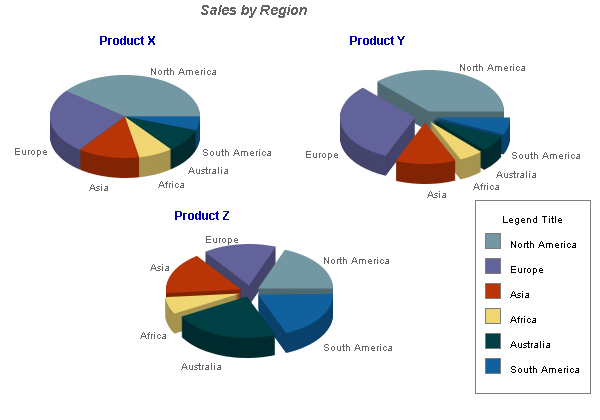
\includegraphics[width=.8\textwidth]{figures/servlet3.png}
  \caption[A Pie chart]{Stolen from the net. Google for a pie chart...}
  \label{fig:pie}
\end{figure}

Many graphics packages can produce pdf files
Embedded postscript (file extension .eps) are also a good candidate,
after converting them to pdf with the epstopdf tool. By the way: the
native format of Adobe Illustrator (ai) is similar enough to eps, so
that too can be processed with ps2pdf. Programs like {\em Visual
  Paradigm} are able to produce pdf files too. And sometimes open-office can
lend a helping hand, for by cutting and pasting Windows graphics into
a single page oodraw drawing, you can produce an very usable pdf file. 

Bitmap file types like png and jpeg take up a lot of space in your
final pdf document. 
Bitmap files take even more space if encoded into a pdf file.
If at all possible, stick to a vector format like eps or pdf (if
necessary derived from eps files). 

%\clearpage%to show headers

\section{A png example}
\label{page:pngexample}
If latex cannot fit the diagram on this page
(page~\pageref{page:pngexample}), 
 then you may find the diagram as figure~\vref{fig:pie}. And as you
 can see, you can easily reference pages and figures.

%\clearpage%to show headers
\section{PDF from an UML package} 
% Note how this varioref expands to
% something like on the next page.
% and using a wrapfigure
\begin{wrapfigure}{r}{.4\textwidth}

  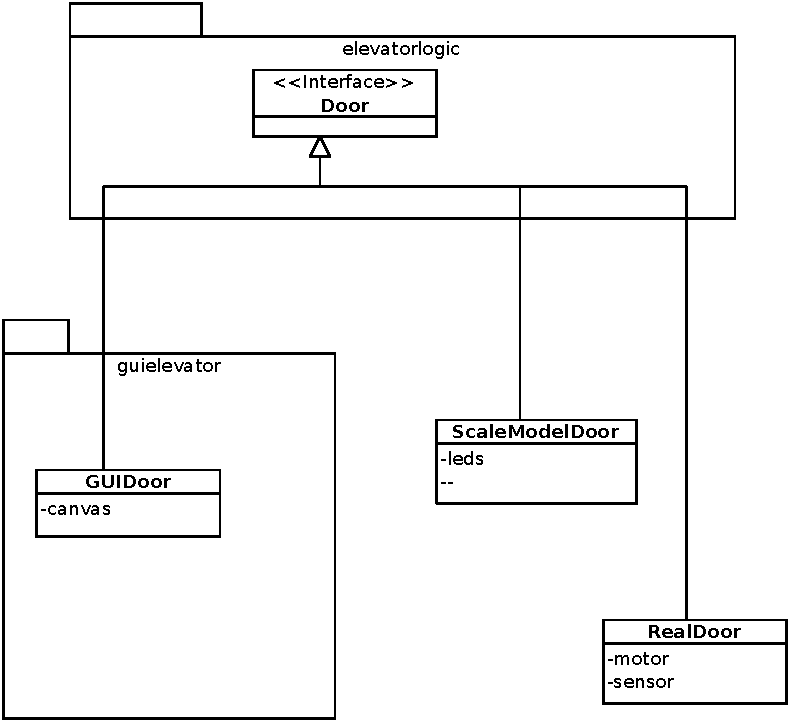
\includegraphics[width=.4\textwidth]{figures/doorsystem.pdf}
  \caption{A class diagram made with Visual Paradigm}
  \label{fig:classdiagram}
\end{wrapfigure}
If the documentation you write is a design document of some software
package, you may want to include design diagrams.
No software engineering without a UML diagrams\ldots.
You can see one generated with ``dia'', a vector drawing program that
understands the UML in figure~\ref{fig:classdiagram}
~\vpageref{fig:classdiagram}. This diagram is 'wrapped' in a \Code{wrapfigure} environment, so the text may flow around it

The diagram is not very sophisticated but shows an example of a vector
format file included via an eps$\rightarrow$ pdf conversion by
epstopdf.

Open source programs like umlet and argouml are also able to produce
vector format graphics files. And sometimes it is helpful to add a box 
that is a bit bigger then the picture you want to include.
This ensures that the so called bounding box does not cut of any lines
you want in your picture. Sometimes it is necessary to give these
tools a helping hand with inkscape, that is do a bit of tinkering to
get all details right.
\begin{figure}[htbp]
  \centering
  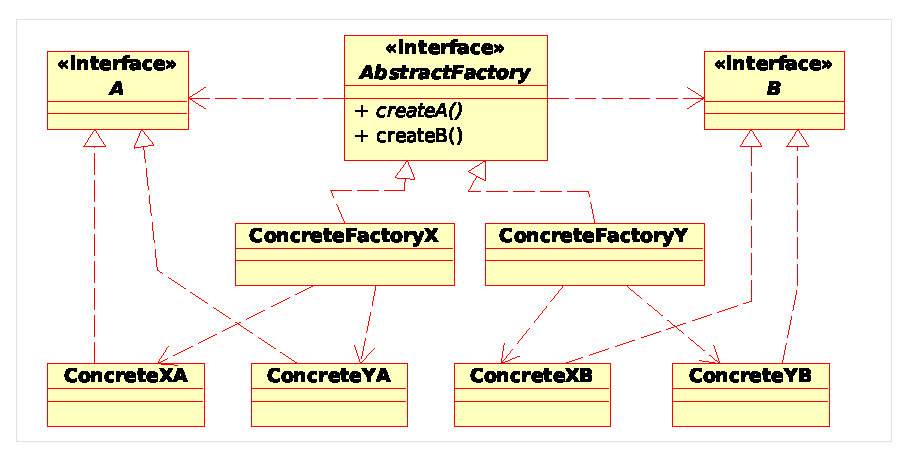
\includegraphics[width=.6\textwidth]{figures/factory}
  \caption[A class diagram by Umbrello]{A class diagram by Umbrello, saved as svg and processed
    with inkscape.}
  \label{fig:factory}
\end{figure}

% On the front cover you can find an ArgoUml diagram that shows how you could
% arrange a set of files, which would allow you to present on screen or on
% paper and in several languages from the same source files. We use this
% to prepare our freshmen syllabi and exams.

%%% Local Variables: 
%%% mode: latex
%%% TeX-master: "main"
%%% End: 

\svnidlong{$HeadURL: https://www.fontysvenlo.org/svnp/879417/latexcolloquium/trunk/latexsample/codelisting.tex $}%
{$LastChangedDate: 2014-11-16 16:03:56 +0100 (zo, 16 nov 2014) $}%
{$LastChangedRevision: 62 $}%
{$LastChangedBy: 879417 $}
\svnid{$Id: codelisting.tex 62 2014-11-16 15:03:56Z 879417 $}
\renewcommand\TheFile{codelistings.tex}

\begin{savequote}[8cm]
  \sffamily
  Use the source Luke.
  \qauthor{The most accurate documentation is in the source.}
  Addendum: Document your source well! And choose proper names.
  \qauthor{Pieter van den Hombergh}
\end{savequote}
\chapter{Listings and code documentation}
For these functions to work you need to use the \texttt{package} listings.
See mydefs.tex for the inclusion.

\lstset{%first some settings
  numbers=right, % number the lines
  numberstyle={\tiny\color{red}},frame=shadowbox,rulesepcolor=\color{gray},
  framexrightmargin=5mm
}

Note that the line numbers in the right hand border are the line
numbers in the included sources.

A good advice is to start using \define{doxygen} for your code documentation.
It can produce nicely formatted HTML and latex documents and can be
tuned in various ways with the  
help of doxywizard. The way of working is a lot like using javadoc,
but also works for C and C++ files. 
See e.g. the documentation on the zthreads package at
\url{http://zthread.sourceforge.net} or Qt at 
\url{http://doc.trolltech.com/3.3/index.html}

\section{Source code}
The most simple case: include the whole thing with a command like \\
\verb#\lstinputlisting[language=java]{code/Hi.java}#
\lstinputlisting[language=java]{code/Hi.java}

Sometimes it is useful to include just a part of a file, for instance
when you want to explain things. Like what line 11 is all about.\\
\verb#\lstinputlisting[language=java, firstline=11,lastline=11]{Hi.java}#
\lstinputlisting[language=java, firstline=11,firstnumber=11,
        lastline=11,numbers=right,basicstyle={\small\ttfamily},
        caption={use toString to let an object represent itself.}
        ]{code/Hi.java}

\section{Makefiles}
You can also include make files.
Note that makefiles have a peculiar syntax. \define{Spaces and tabs in
  Makefiles}\ are meaningful. 
That's why I made them show up in the next listing with the command\\
\lstinputlisting[firstline=65,lastline=67]{codelisting.tex}
\lstset{showspaces=true,showtabs=true}
Spaces show up as \lstinline| |, tab characters as an extended version
of the same thing (\lstinline|	|). 
As can be expected, spaces and tabs have no special meaning in
makefile comments, the lines starting with a hash (\#) sign. 
If you want to know more on makefiles try google or info:make in
konqueror on a decently installed Linux box.  

The make file for this entire document looks like this:
\lstinputlisting[language=make,showtabs=true,
     showspaces=true,basicstyle={\ttfamily\scriptsize},
     numbers=right,language=make]{Makefile}


%%% Local Variables: 
%%% mode: latex
%%% TeX-master: "main"
%%% End: 

\svnidlong{$HeadURL: https://www.fontysvenlo.org/svnp/879417/latexcolloquium/trunk/latexsample/poser.tex $}%
{$LastChangedDate: 2013-09-08 12:54:29 +0200 (Sun, 08 Sep 2013) $}%
{$LastChangedRevision: 31 $}%
{$LastChangedBy: 879417 $}
\svnid{$Id: poser.tex 31 2013-09-08 10:54:29Z 879417 $}
\renewcommand\TheFile{poser.tex}
\begin{savequote}[8cm]
  \sffamily
  Never start reading a difficult book at the wrong side.\\ 
  It makes you feel stupid.
  \qauthor{Private experience}
\end{savequote}
\chapter{So {\em you}\ know how to show off, but how do {\em I}\
  start?} 

\lstset{numberstyle={\tiny\color{red}},
  basicstyle={\small},numbers=right,
  rulesepcolor=\color{gray},
  showspaces=false,frame=shadowbox}

This document is indeed a bit of a showcase, but there is more to it.
In essence, most documents are mainly texts. 
And those plain texts take mainly typing and not much more.
The minimal, hello world style \LaTeX\ file is not much 
longer\footnote{Counting headers too!} then the C classic.
\lstinputlisting[firstline=5]{simple.tex}

And the pictures, well they are made with other packages, and as long
as those can produce a supported format, you can use them. \TeX\ and
\LaTeX\ have an own drawing language, but explaining that would blow
up this space.
There is a lot of documentation available on \TeX\ and \LaTeX\ and I
could recommend some good books on it.
But you need not run off to the nearest book shop. Lots of
documentation is on the Net, just as the \TeX\ program suite itself. 

Look for instance at \url{http://www.ntg.nl} for the Dutch \TeX\ user group
and \url{http://www.dante.de} for the German user group. They are both very 
alive and kicking.

A very good starting point nowadays is \url{http://en.wikibooks.org/wiki/LaTeX/}

\section{My own definitions}
Standard \LaTeX\ output looks a bit dull but are nicely formatted nonetheless.
If you want to make the most of your own style for your own or your
projects documentation, put your style definitions into a separate
file. That way you can keep all definitions of style and \define{macros} in one
spot. This works especially nicely in an multi part document, so
the other files (and authors) can concentrate on content.

You can \define{define} your own macros in \LaTeX. As an example a macro,
\verb#\define#, which I use
to let words stand out at the outer margin. I use it at the first use
of a word or concept in the text, to aid the reader in finding the
definition. Of course this macro could be extended to put the word
into an index. Which makes it a nice exercise.
The macro is defined as follows:\\
\lstinputlisting[frame=shadowbox,firstline=70,lastline=77]{mydefs.tex}

and is used as \verb#\define{new word}#.


%%% Local Variables: 
%%% mode: latex
%%% TeX-master: "main"
%%% End: 

\svnidlong{$HeadURL: https://www.fontysvenlo.org/svnp/879417/latexcolloquium/trunk/latexsample/programmedgraphics.tex $}%
{$LastChangedDate: 2013-09-08 12:54:29 +0200 (Sun, 08 Sep 2013) $}%
{$LastChangedRevision: 31 $}%
{$LastChangedBy: 879417 $}
\svnid{$Id: programmedgraphics.tex 31 2013-09-08 10:54:29Z 879417 $}
\renewcommand\TheFile{programmedgraphics.tex}
\begin{savequote}[8cm]
 \sffamily
  A drawing created with just a few words.\\ 
  Or the old adagium 'a thousand words' reversed.
  \qauthor{Private experience}
\end{savequote}
\chapter{Drawing in \LaTeX}

There are quite a few developers who add usefull packages to 
the \TeX world. One of them is Till Tantau of the ``Technische
Üniversität'' in Berlin Germany. He produced the package called pgf,
which stands for portable graphics format. 


The pgf package contains the macro tool \texttt{tikz}, that allows you to draw 
quite nice graphics with just a few commands. Like this small ellipse:
\tikz \draw[rotate=30] (0,-1) ellipse (5pt and 3pt);

The pgf manual has many nice examples that may prove usefull,
certainly if you want to use the package beamer\footnote{also by Till
  Tantau} to create professional looking pdf presentations with \LaTeX.

A simple figure from the pgf manual:

\begin{figure}[htbp]
\begin{tikzpicture}[scale=2,cap=round]
  % Local definitions
  \def\costhirty{0.8660256}

  % Colors
  \colorlet{anglecolor}{green!50!black}
  \colorlet{sincolor}{red}
  \colorlet{tancolor}{orange!80!black}
  \colorlet{coscolor}{blue}

  % Styles
  \tikzstyle{axes}=[]
  \tikzstyle{important line}=[very thick]
  \tikzstyle{information text}=[rounded corners,fill=red!10,inner sep=1ex]

  % The graphic
  \draw[style=help lines,step=0.5cm] (-1.4,-1.4) grid (1.4,1.4);
  
  \draw (0,0) circle (1cm);

  \begin{scope}[style=axes]
    \draw[->] (-1.5,0) -- (1.5,0) node[right] {$x$} coordinate(x axis);
    \draw[->] (0,-1.5) -- (0,1.5) node[above] {$y$} coordinate(y axis);

    \foreach \x/\xtext in {-1, -.5/-\frac{1}{2}, 1}
      \draw[xshift=\x cm] (0pt,1pt) -- (0pt,-1pt) node[below,fill=white] {$\xtext$};
  
    \foreach \y/\ytext in {-1, -.5/-\frac{1}{2}, .5/\frac{1}{2}, 1}
      \draw[yshift=\y cm] (1pt,0pt) -- (-1pt,0pt) node[left,fill=white] {$\ytext$};
  \end{scope}
    
  \filldraw[fill=green!20,draw=anglecolor] (0,0) -- (3mm,0pt) arc(0:30:3mm);
  \draw (15:2mm) node[anglecolor] {$\alpha$};
    
  \draw[style=important line,sincolor]
    (30:1cm) -- node[left=1pt,fill=white] {$\sin \alpha$} (30:1cm |- x axis);
  
  \draw[style=important line,coscolor]
    (30:1cm |- x axis) -- node[below=2pt,fill=white] {$\cos \alpha$} (0,0);
  
  \draw[style=important line,tancolor] (1,0) -- node[right=1pt,fill=white] {
    $\displaystyle \tan \alpha \color{black}=
    \frac{{\color{sincolor}\sin \alpha}}{\color{coscolor}\cos \alpha}$}
    (intersection of 0,0--30:1cm and 1,0--1,1) coordinate (t);

  \draw (0,0) -- (t);
  
  \draw[xshift=1.85cm]
    node[right,text width=6cm,style=information text]
    {
      The {\color{anglecolor} angle $\alpha$} is $30^\circ$ in the
      example ($\pi/6$ in radians). The {\color{sincolor}sine of
        $\alpha$}, which is the height of the red line, is
      \[
      {\color{sincolor} \sin \alpha} = 1/2.
      \]
      By the Theorem of Pythagoras ...
    };
\end{tikzpicture}
\caption[A pgf/Tikz drawing]{A drawing taken from the pgf
  manual/tutorial by Till Tantau}
\label{fig:tikz}
\end{figure}


%%% Local Variables: 
%%% mode: latex
%%% TeX-master: "main"
%%% End: 

\begin{savequote}[.4\textwidth]
\sffamily
Everything should be made as simple as possible, but not simpler.
\qauthor{Albert Einstein}
\end{savequote}
\chapter{Citing is simple}

Adding proper references and citations to you document can be a real
burden.
Not so in \LaTeX\ where you can use the facilities of a kind ``database''
and many entries available on the web that be added to that database.

This database can be one file, but just as well a set of files, which
you use to organize you bibliography. The files with these data are
called .bib files. 

\section{bibtex}
Using bibtex is easy.
For instance if your bib contains this entry \citep{bibtexsite}
\begin{lstlisting}[language=BibTeX]
@misc{ Nobody06,
       author = "Nobody Jr",
       title = "My Article",
       year = "2006" }
\end{lstlisting}
\lstset{language=BibTeX}
Then citing Nobody~\cite{Nobody06} is easy as
pie:\lstinline|\cite{Nobody06}|

Then you need to add one compilation step to your normal workflow:

\begin{lstlisting}[language=sh]
$ latex myarticle
$ bibtex myarticle
$ latex myarticle
$ latex myarticle
\end{lstlisting}

You can of course easily add that to the makefile introduced in an
earlier chapter.

Bibtex is the standard you want to use if preparing an article of a
journal or magazine. The journal typically also prescribes a specific
bibliography style (defined in a .bst file), which is most likely
already define for or by that journal

\subsection{Biblatex and biber}
A bit more modern is biblatex, which has a much simpler definition
format for bst files. The is a separate \textbf{biber} program to do
the processing instead of the bibtex run.
I have used biber in this version of this latex sample.


\lstlistoflistings
\addcontentsline{toc}{chapter}{References}
\printbibliography[title={\color{gray}References}]

\clearpage
\def\BackCoverMaterial{
  \setlength{\unitlength}{1mm}
  \begin{center}

  \vspace{.3\paperheight}
  \begin{picture}(160,160)
%  \begin{minipage}{\textwidth}
    \put(10,10){
\includegraphics[width=120mm]{figures/TheEnd.jpg}}
%  \end{minipage}
  \end{picture}
\end{center}
\vfill
}


\end{document}
